\documentclass[twoside,12pt]{article}
%\documentclass{book}

\setcounter{secnumdepth}{5}

\usepackage[nottoc]{tocbibind}
\usepackage[toc,page]{appendix}
\usepackage{amsmath,amsfonts,amsthm,fullpage}
\usepackage{amsmath}
\usepackage{amssymb}
\usepackage{listings}
\setlength{\parindent}{0pt}
\usepackage{graphicx}
\usepackage{bm}
\usepackage[section]{placeins}
\usepackage{lipsum} % just for the example
\usepackage{array}
\usepackage[export]{adjustbox}
\usepackage{subfigure}
\usepackage{titlesec}
\usepackage{multirow}
\usepackage[section]{placeins}
\usepackage{tabularx} 
\usepackage{mathtools}
\usepackage[nodisplayskipstretch]{setspace}
\usepackage{color}
% Use the standard article template.
%
% The geometry package allows for easy page formatting.
\usepackage{geometry}
% Load up special logo commands.
\usepackage{doc}
% Package for formatting URLs.
\usepackage{url}
% Packages and definitions for graphics files.
\usepackage{epstopdf}



%
\geometry{letterpaper}
\setstretch{1}

\DeclareGraphicsRule{.tif}{png}{.png}{`convert #1 `dirname #1`/`basename #1 .tif`.png}

\def\argmin{\operatornamewithlimits{arg\, min}}
\newcommand{\rbr}[1]{\left(#1\right)}
\newcommand{\cbr}[1]{\left\{#1\right\}}
\newcommand{\Ncal}{\mathcal{N}}
\renewcommand{\familydefault}{\sfdefault}
\newcolumntype{L}{>{\centering\arraybackslash}m{3cm}}
\def\argmin{\operatornamewithlimits{arg\, min}}
%\newcommand\Myperm[2][n]{\prescript{#1\mkern-2.5mu}{}P_{#2}}
%\newcommand\Mycomb[2][n]{\prescript{#1\mkern-0.5mu}{}C_{#2}}
\newcommand\inv[1]{#1\raisebox{1.15ex}{$\scriptscriptstyle-\!1$}}
\newcommand\numberthis{\addtocounter{equation}{1}\tag{\theequation}}
\newcommand{\norm}[1]{\left\lVert #1 \right\rVert}
%\newcommand{\tendsto}[1]{%\xrightarrow{\smash{\raisebox{-2ex}{$\scriptstyle#1$}}}}


\definecolor{dkgreen}{rgb}{0,0.6,0}
\definecolor{gray}{rgb}{0.5,0.5,0.5}
\definecolor{mauve}{rgb}{0.58,0,0.82}

\lstset{frame=tb,
  language=Java,
  aboveskip=3mm,
  belowskip=3mm,
  showstringspaces=false,
  columns=flexible,
  basicstyle={\small\ttfamily},
  numbers=none,
  numberstyle=\tiny\color{gray},
  keywordstyle=\color{blue},
  commentstyle=\color{dkgreen},
  stringstyle=\color{mauve},
  breaklines=true,
  breakatwhitespace=true,
  tabsize=3
}


\setcounter{secnumdepth}{4}
\titleformat{\paragraph}
{\normalfont\normalsize\bfseries}{\theparagraph}{1em}{}
\titlespacing*{\paragraph}
{0pt}{3.25ex plus 1ex minus .2ex}{1.5ex plus .2ex}


\titlespacing\section{0pt}{2pt plus 1pt minus 1pt}{0pt plus 1pt minus 1pt}
\titlespacing\subsection{0pt}{2pt plus 1pt minus 1pt}{0pt plus 1pt minus 1pt}
\titlespacing\subsubsection{0pt}{2pt plus 1pt minus 1pt}{0pt plus 1pt minus 1pt}
\allowdisplaybreaks



%
% Set the title, author, and date.
%
\title{Iterative Solution to a Non Linear System }
\author{Ajay D'Souza (adsouza31)}
\author{
  D'Souza, Ajay\\
  \texttt{ajaydsouza@gatech.edu}
}
\date{}
  
\iffalse
*------------------------------------------------------------*
  These are the instructions for the Final Report
*------------------------------------------------------------*

\fi

\begin{document}

\maketitle
\begin{center}
Newtons Method to solve a system of non linear equations from the discretization of a Laplacian Boundary Value Problem
\end{center}

% Add an abstract.
\begin{abstract}
To Solve the given boundary value problem  - An application in Physical Sciences. Formulate it as a problem of a system of equations and solve it using an appropriate iterative process for solving that system of equations
\end{abstract}
% Add various lists on new pages.
\pagebreak
\tableofcontents

\pagebreak
\listoffigures
\listoftables

% Start the paper on a new page.
\pagebreak



%
% Body text.
%
$\\\\$
\section{Introduction}
\label{intro}
The problem is an application in physical sciences problem of finding a path from one local optima to another due to noise under certain specified conditions. This is treated as a boundary value problem. We reformulate this problem using discretization as a solution to a system of equations. A closer examination of the formulation, reveals it to be a non linear system. We use Newtons method which is an iterative method ,to attempt to solve this system of non linear equations. 


$\\\\$
\section{Method}
\label{method}

We are given,
\begin{align*}
X &= \begin{bmatrix}x\\y\end{bmatrix}\\\\
V(X) &= \frac{(1-x^2)^2}{4} + \frac{(y+x^2-1)^2}{2}
\end{align*}

We determine,
\begin{align*}
\nabla V(X) &= \begin{bmatrix}
\frac{dV(X)}{dx}\\\\\frac{dV(X)}{dy}
\end{bmatrix}\\
&= \begin{bmatrix}
-x(1-x^2)+2x(y+x^2-1)\\\\
y+x^2-1
\end{bmatrix}\\
\\
\\
HessV(X) &= \begin{bmatrix}
H_{11} & H_{12}\\\\
H_{21}& H_{22}
\end{bmatrix}\\\\
&=\begin{bmatrix}
\frac{d^2 V(X)}{dx^2} & \frac{d^2 V(X)}{dx dy}\\\\
\frac{d^2 V(X)}{dy dx}& \frac{d^2V(X)}{dy^2}
\end{bmatrix}\\\\
&= \begin{bmatrix}
(2y+9x^2-3)&2x\\\\
2x&1
\end{bmatrix}
\end{align*}


The Boundary Value Problem to Solve is
\begin{align*}
X^{''}(t) &= HessV(X(t)) \nabla V(X(t)) \numberthis\label{p1_1}\\
\;\;\;\text{,with}\;\;\;X(0)&=X_a=\begin{bmatrix}-1\\0\end{bmatrix},\\
\;\;\;X(T)&=X_b=\begin{bmatrix}1\\0\end{bmatrix}
\end{align*}

Where $X= \begin{bmatrix}x\\y\end{bmatrix}$, and $F\colon \mathbb{R}^2\to\mathbb{R}^2$, The RHS of $\eqref{p1_1}$ can be expressed as
\begin{align*}
HessV(X) \nabla V(X)
  &= F(X)\numberthis\label{p1_2}\\\\
  &= \begin{bmatrix}
\frac{d^2 V(X)}{dx^2} & \frac{d^2 V(X)}{dx dy}\\\\
\frac{d^2 V(X)}{dy dx}& \frac{d^2V(X)}{dy^2}
\end{bmatrix} \times \begin{bmatrix}
\frac{dV(X)}{dx}\\\\\frac{dV(X)}{dy}
\end{bmatrix}  \\
\\
 &= \begin{bmatrix}
 (2y+9x^2-3)&2x\\
 2x&1
 \end{bmatrix} \times \begin{bmatrix}
 -x(1-x^2)+2x(y+x^2-1)\\
 y+x^2-1
 \end{bmatrix}  \\
\\
&=  \begin{bmatrix}
 (2y+9x^2-3)(-x(1-x^2)+2x(y+x^2-1))+2x(y+x^2-1)\\
 2x(-x(1-x^2)+2x(y+x^2-1))+(y+x^2-1)
 \end{bmatrix}\\
 \\
 &=  \begin{bmatrix}
  27x^5-34x^3+7x+24x^3y+4xy^2-10xy\\
  6x^4-5x^2+4x^2y+y-1
  \end{bmatrix}
 \end{align*}

 The Laplace Operator on the LHS of $\eqref{p1_1}$ , $\Delta X$ can be discretized at $t = i$ using central difference approximation as
 \begin{align*}
X^{''}(t) &= \begin{bmatrix}
 \frac{d^2x}{dt^2}\\\\
 \frac{d^2y}{dt^2}
 \end{bmatrix} \\ &=  \Delta X_{i} \\
 &=  \frac{X_{(i+h)}+X_{(i-h)}-2X_{(i)}}{h^2}, \numberthis\label{p1_3}\\
 &\text{where,}\\
 h &= \frac{T}{M},\\
 i &\in 1\dots(M-1)\\
 X_i&= \begin{bmatrix}x_i\\y_i\end{bmatrix}
 \end{align*}


Using $\eqref{p1_2}$ and  $\eqref{p1_3}$ in $\eqref{p1_1}$ , and again using the fact that $X_i= \begin{bmatrix}x_i\\y_i\end{bmatrix}$, and $F\colon \mathbb{R}^2\to\mathbb{R}^2$,  we can express the boundary value problem to be solved in terms of a system of non linear equations as
\begin{align*}
\frac{X_{(i+h)}+X_{(i-h)}-2X_{(i)}}{h^2} &= F(X_i)\\
\;\;\;\text{,with}\;\;\;X(0)&=X_a=\begin{bmatrix}-1\\0\end{bmatrix},\\
X(T)&=X_b=\begin{bmatrix}1\\0\end{bmatrix}\\
h &= \frac{T}{M},\\
i &\in 1\dots(M-1)\\
\\\\
\implies \frac{1}{h^2}\bigg(\begin{bmatrix}x_{i+h}\\y_{i+h}\end{bmatrix}+\begin{bmatrix}x_{i-h}\\y_{i-h}\end{bmatrix}-2\begin{bmatrix}x_{i}\\y_{i}\end{bmatrix}\bigg) &= F(X_i)\\
\text{,with}\;\;\;\begin{bmatrix}x_{0}\\y_{0}\end{bmatrix}&=\begin{bmatrix}-1\\0\end{bmatrix},\\
\begin{bmatrix}x_{M}\\y_{M}\end{bmatrix}&=\begin{bmatrix}1\\0\end{bmatrix}\\
h &= \frac{T}{M}\\
i &\in 1\dots(M-1)\\
\\\\
\implies \begin{bmatrix}-x_{i-h}+2 x_i -x_{i+h}\\-y_{i-h}+2 y_i -y_{i+h}
 \end{bmatrix} &=  - h^2 F(X_i)\numberthis\label{p1_4}\\
\text{,with}\;\;\;\begin{bmatrix}x_{0}\\y_{0}\end{bmatrix}&=\begin{bmatrix}-1\\0\end{bmatrix},\\
\begin{bmatrix}x_{M}\\y_{M}\end{bmatrix}&=\begin{bmatrix}1\\0\end{bmatrix}\\
h &= \frac{T}{M}\\
i &\in 1\dots(M-1)\\
\end{align*}
From $\eqref{p1_4}$,  and where $X_i= \begin{bmatrix}x_i\\y_i\end{bmatrix}$, and $F\colon \mathbb{R}^2\to\mathbb{R}^2$ we can express the system of equations for different values of $i \in 1\dots(M-1)$ as
\begin{align*}
\intertext{For i=1}
\begin{bmatrix}-x_{0}+2 x_1 -x_{2}\\-y_{0}+2 y_1 -y_{2}
 \end{bmatrix} &=  - h^2F(X_1)\\
\begin{bmatrix}2 x_1 -x_{2}\\2 y_1 -y_{2}
 \end{bmatrix} &= \begin{bmatrix}-1\\0\end{bmatrix} - h^2 F(X_1) \numberthis\label{p1_5}
 \\
\intertext{For any $i \in 2\dots M-2$}
\begin{bmatrix}-x_{i-1}+2 x_i -x_{i+1}\\-y_{i-1}+2 y_i -y_{i+1}
 \end{bmatrix} &= - h^2F(X_i)\numberthis\label{p1_6}
\\
\intertext{For i=M-1}
\begin{bmatrix}-x_{M-2}+2 x_{M-1} -x_{M}\\-y_{M-2}+2 y_{M-1} -y_{M}
 \end{bmatrix} &= - h^2F(X_{M-1})\\
\begin{bmatrix}-x_{M-2} + 2 x_{M-1} \\-y_{M-2} + 2 y_{M-1} 
 \end{bmatrix} &= \begin{bmatrix}1\\0\end{bmatrix} -  h^2 F(X_{M-1})\numberthis\label{p1_7}
\end{align*}
Using $\eqref{p1_5}$, $\eqref{p1_6}$ and $\eqref{p1_7}$, we can write the LHS and RHS of $\eqref{p1_1}$ in matrix form as 
\begin{align*}
\begin{bmatrix}
2&0&-1\\
0&2&0&-1\\
-1&0&2&0&-1\\
0&-1&0&2&0&-1\\
\dots\\
\dots\\
\dots\\
\dots\\
\dots\\
\dots\\
0&&&\dots&-1&0&2&0&-1&0\\
0&&&\dots&&-1&0&2&0&-1\\
0&&&\dots&&&-1&0&2&0\\
0&&&\dots&&&&-1&0&2\\
\end{bmatrix}
 \times \begin{bmatrix}
x_1\\y_1\\x_2\\y_2\\x_2\\y_3\\.\\.\\x_{M-3}\\y_{M-3}\\x_{M-2}\\y_{M-2}\\x_{M-1}\\y_{M-1}\end{bmatrix} &=  \begin{bmatrix}
-1\\0\\0\\0\\0\\0\\.\\.\\0\\0\\0\\0\\1\\0\end{bmatrix} + -h^2 \begin{bmatrix} \begin{bmatrix}F(X_1)[1]\\F(X_1)[2]\end{bmatrix} \\
\begin{bmatrix}F(X_2)[1]\\F(X_2)[2]\end{bmatrix}\\
\begin{bmatrix}F(X_3)[1]\\F(X_3)[2]\end{bmatrix}\\.\\.\\
\begin{bmatrix}F(X_{M-3})[1]\\F(X_{M-3})[2]\end{bmatrix}\\
\begin{bmatrix}F(X_{M-2})[1]\\F(X_{M-2})[2]\end{bmatrix}\\
\begin{bmatrix}F(X_{M-1})[1]\\F(X_{M-1})[2]\end{bmatrix}\end{bmatrix} \numberthis\label{p1_8}
\end{align*}
Where,
\begin{flalign*}
h = \frac{T}{M}\\
G\colon \mathbb{R}^2\to\mathbb{R}^2\\
F(X)=  \begin{bmatrix}
  27x^5-34x^3+7x+24x^3y+4xy^2-10xy\\
  6x^4-5x^2+4x^2y+y-1
  \end{bmatrix}\\
\begin{bmatrix}x_{0}\\y_{0}\end{bmatrix}=\begin{bmatrix}-1\\0\end{bmatrix},\;\begin{bmatrix}x_{M}\\y_{M}\end{bmatrix}=\begin{bmatrix}1\\0\end{bmatrix}\\
\end{flalign*}
$\eqref{p1_8}$ is a system of non linear equations since  $F(X)$ is non linear in $X$. So this needs to be solved as a system of non linear equations. We can express $\eqref{p1_8}$ in a simpler matrix notation as 
\begin{align*}
 AX +h^2 F(X,z) - \hat{Y} &= 0\numberthis\label{p1_9}\\
 \intertext{Where,}
 A_{2(M-1)\times2(M-1)} &= \begin{bmatrix}
 2&0&-1\\
 0&2&0&-1\\
 -1&0&2&0&-1\\
 0&-1&0&2&0&-1\\
 \dots\\
 \dots\\
 \dots\\
 \dots\\
 \dots\\
 \dots\\
 0&&&\dots&-1&0&2&0&-1&0\\
 0&&&\dots&&-1&0&2&0&-1\\
 0&&&\dots&&&-1&0&2&0\\
 0&&&\dots&&&&-1&0&2\\
 \end{bmatrix}\\
 X_{2(M-1)} &= \begin{bmatrix}
 x_1\\y_1\\x_2\\y_2\\x_2\\y_3\\.\\.\\x_{M-3}\\y_{M-3}\\x_{M-2}\\y_{M-2}\\x_{M-1}\\y_{M-1}\end{bmatrix}\\
 \hat{Y}_{2(M-1)} &= \begin{bmatrix}
 -1\\0\\0\\0\\0\\0\\.\\.\\0\\0\\0\\0\\1\\0\end{bmatrix} \\
 F(X,z)_{2(M-1)} &=  \begin{bmatrix} \begin{bmatrix}F(X_1)[1]\\F(X_1)[2]\end{bmatrix} \\\begin{bmatrix}F(X_2)[1]\\F(X_2)[2]\end{bmatrix}\\
 \begin{bmatrix}F(X_3)[1]\\F(X_3)[2]\end{bmatrix}\\.\\.\\\begin{bmatrix}F(X_{M-3})[1]\\F(X_{M-3})[2]\end{bmatrix}\\\begin{bmatrix}F(X_{M-2})[1]\\F(X_{M-2})[2]\end{bmatrix}\\\begin{bmatrix}F(X_{M-1})[1]\\F(X_{M-1})[2]\end{bmatrix}\end{bmatrix}
 \intertext{Let,}
 G(X,z) &= AX +h^2 F(X,z) - \hat{Y}
 \intertext{Then at $X_i$, we can express X in a linear form in G as}
 X &= X_k - \inv{[\mathbb{J}(X_i,z)]} G(X_i,z) \\
 X &= X_k - \inv{[\mathbb{J}(X_i,z)]} (AX_i +h^2 F(X_i,z) - \hat{Y}) \numberthis\label{p1_10}
 \intertext{The Jacobi Matrix $\mathbb{J}(X_i,z)$ is on $ G(X_i,z)$, so it can be computed as,}
 \mathbb{J}(X,z) &= \frac{dG(X,z)}{dX}\\
 &= \frac{d(AX +h^2 F(X,z) - \hat{Y})}{dX}\\
 \therefore \mathbb{J}(X,z) &= A+ h^2 \mathbb{J_F}(X,z)\numberthis\label{p1_11}
 \intertext{Using $\eqref{p1_11}$ in $\eqref{p1_10}$ we get }
 X & = X_k - \inv{[ A+ h^2 \mathbb{J_F}(X_i,z)]} (AX_i +h^2 F(X_i,z) - \hat{Y}) \numberthis\label{p1_12}
\end{align*}
The Jacobian Matrix $\mathbb{J_F}(X_i,z)$ on $F(X,z)$ can be computed as below
\begin{align*}
\mathbb{J_F}(X_i,z) &=\begin{bmatrix}
\frac{dF_{11}}{dx_1}&\frac{dF_{11}}{dy_1}&\\
\frac{dF_{12}}{dx_1}&\frac{dF_{12}}{dy_1}&0&\\
0&0&\frac{dF_{21}}{dx_2}&\frac{dF_{21}}{dy_2}&0\\
0&0&\frac{dF_{22}}{dx_2}&\frac{dF_{22}}{dy_2}&0&0\\
\dots\\
\dots\\
0&&&\dots&0&0&\frac{dF_{(M-2)1}}{dx_{M-2}}&\frac{dF_{(M-2)1}}{dy_{M-2}}&0&0\\
0&&&\dots&&0&\frac{dF_{(M-2)2}}{dx_{M-2}}&\frac{dF_{(M-2)2}}{dy_{M-2}}&0&0\\
0&&&\dots&&&&0&\frac{dF_{(M-1)1}}{dx_{M-1}}&\frac{dF_{(M-1)1}}{dy_{M-1}}\\
0&&&\dots&&&&0&\frac{dF_{(M-1)2}}{dx_{M-1}}&\frac{dF_{(M-1)2}}{dy_{M-1}}\\
\end{bmatrix}
\intertext{Where,}
\frac{dF_{k1}}{dx_k} &= 135x_k^4 - 102x_k^2 + 7 + 72x_k^2y_k + 4y_k^2-10y_k\\
\frac{dF_{k2}}{dx_k} &= 24x_k^3 - 10x_k + 8x_ky_k\\
\frac{dF_{k1}}{dy_k} &= 24x_k^3 + 8x_ky_k - 10x_k\\
\frac{dF_{k2}}{dy_k} &= 4x_k^2 + 1
\end{align*}
\begin{itemize}
\item
Thus we can solve this system of non linear equations by the performing iterations on $\eqref{p1_12}$. 
\item
This is the Newtons Method. 
\item
We perform iterations till the residue $(AX_i +h^2 F(X_i,z) - \hat{Y})$ is below a certain tolerance
\item
We being the iteration by taking an initial  guess value for $X$. For this particular problem we begin with an initial guess zero vector of of $X_{2\times(M-1)} = \begin{bmatrix}0\\.\\,\\0\end{bmatrix}$
\item
The Newtons method is performed for values of T = $[1,5,10,20,100]$
\item
The Newtons Method will use an value of $h=0.1$, where $h$ is the time interval.
\item
The MATLAB source code for this implementation is in file $project\_p\_1\_newtons.m$. The code is also  in the appendix at $\eqref{newtons_source}$
\item
The results of the Newtons Method are plotted in R. The R source code used for plotting is in file $project\_p\_1\_plot\_csv\_results.R$. The code is also in the appendix $\eqref{plotting_source}$
\end{itemize}


\pagebreak
\FloatBarrier
$\\\\$
\section{Results}
\label{results}

\FloatBarrier
\subsection{T=1}
{
The following figure $\eqref{fig:proj_1_g_t_1}$ plots the results of the Newtons method for $T=1$. Full convergence is achieved in 303 iterations. While $x$ moves from $(-1 \to 1)$, $y$ ranges from $0 \to 0.125 \to 0$ during the course of this iteration. The 3D surface plot of $V(x,y) =  \frac{(1-x^2)^2}{4} + \frac{(y+x^2-1)^2}{2}$ for this range of $x,y$ clearly shows the two local minimums at $[-1;0]$ and $[1;0]$ . The $x(t),y(t)$ plot for this iteration shows the path taken by this iteration from $[-1;0] \to [1;0]$
\begin{figure}[htbp!]
     \begin{center}
            \hspace*{-1.4in}           
                    \subfigure[]{%
                        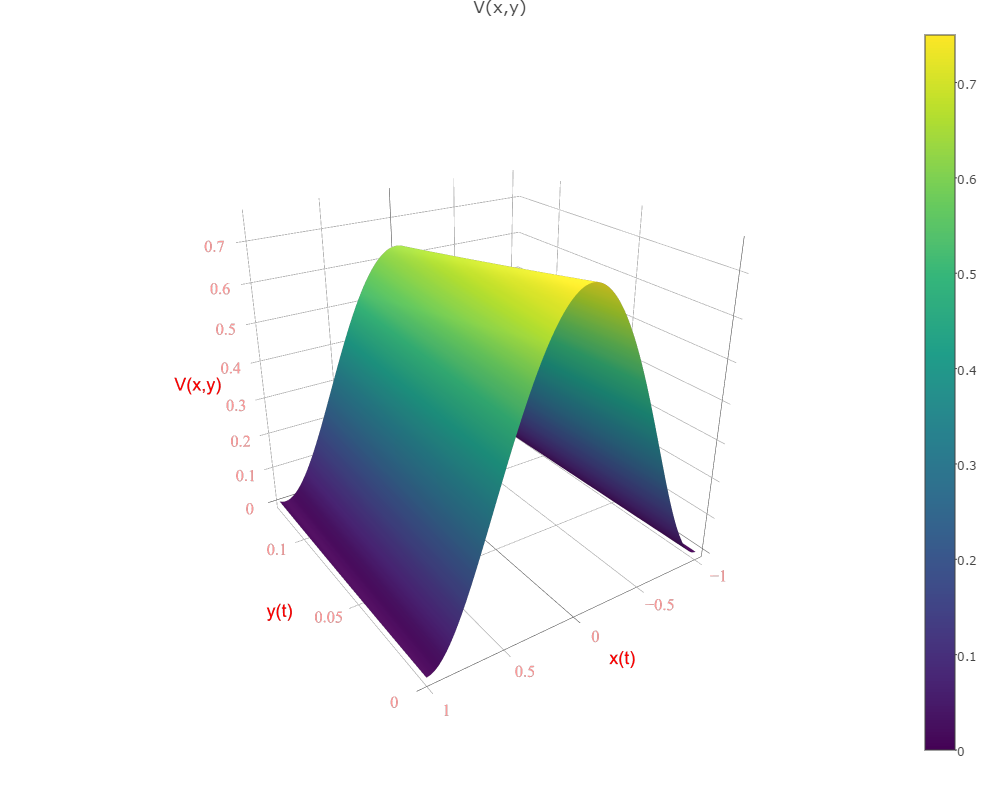
\includegraphics[width=1.05\textwidth]{project_1_g_5_1}
                    }\\%
                    \subfigure[]{%
                    \hspace*{-1.6in}   
                       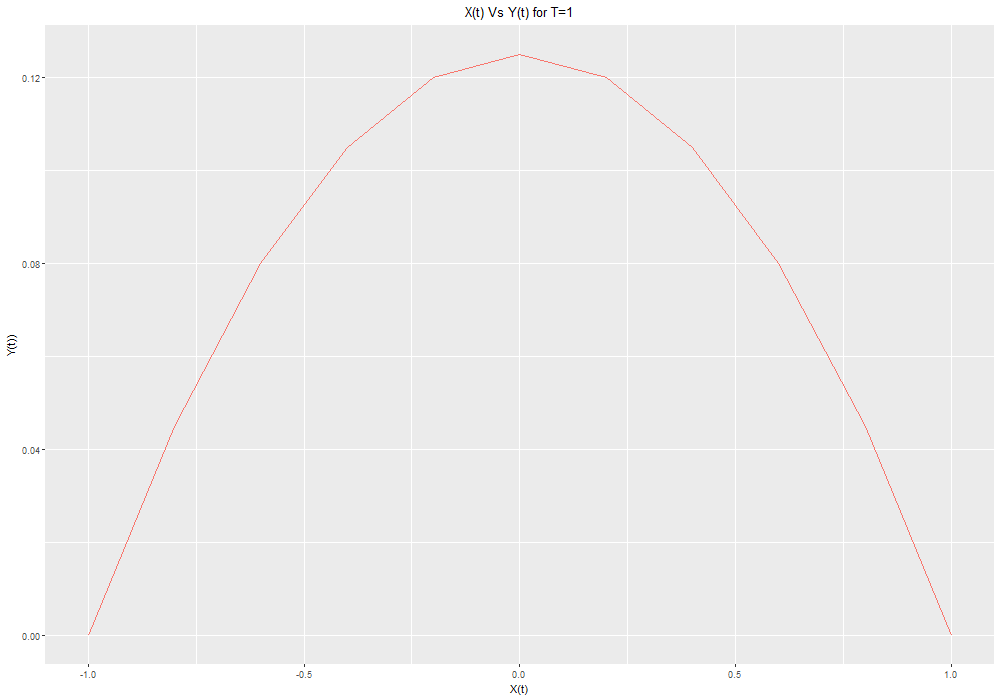
\includegraphics[width=0.8\textwidth]{proj_1_g_xy_t_1}
                    }\\ %  ------- End of the first row ----------------------%
    \end{center}
    \caption{%
     Plot of V(X,Y) Vs X(t)Y(t) and the plot of the solution x(t),y(t) for T=1
     }%
   \label{fig:proj_1_g_t_1}
\end{figure}
}

\FloatBarrier
\subsection{T=5}
{
The figure $\eqref{fig:proj_1_g_t_5}$ plots the iteration results for $T=5$. Full convergence is achieved in 7380 iterations. While $x$ moves from $(-1 \to 1)$, $y$ takes a longer path from $0 \to 3.125 \to 0$ for this iteration. The 3D surface plot of $V(x,y) =  \frac{(1-x^2)^2}{4} + \frac{(y+x^2-1)^2}{2}$ for this range of $x,y$ clearly shows the two local minimums at $[-1;0]$ and $[1;0]$ . The $x(t),y(t)$ plot for this iteration shows the longer path taken by this iteration from $[-1;0] \to [1;0]$
\begin{figure}[htbp!]
     \begin{center}
            \hspace*{-1.4in}           
                    \subfigure[]{%
                        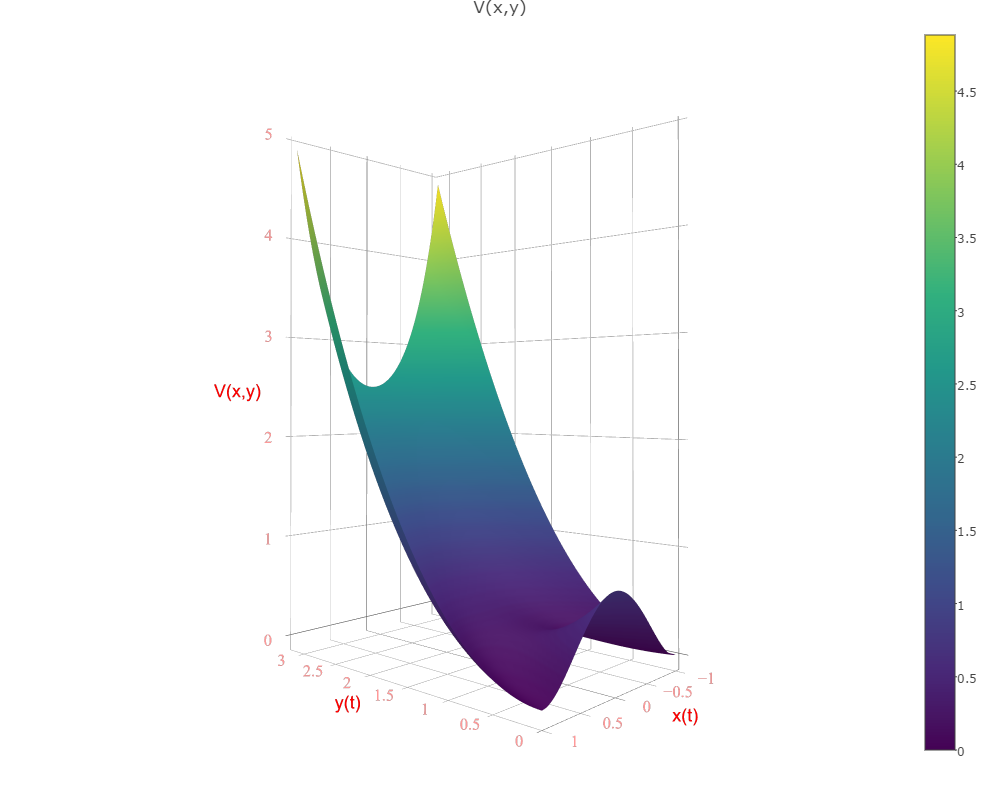
\includegraphics[width=1.0\textwidth]{project_1_g_5_2}
                    }\\%
                    \subfigure[]{%
                    \hspace*{-1.6in}   
                       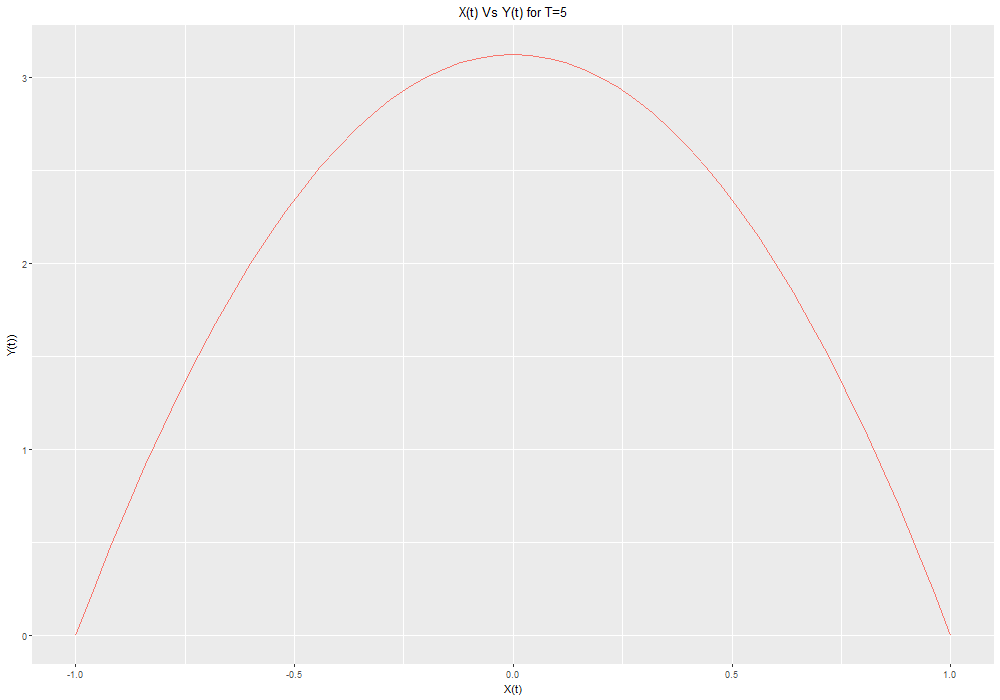
\includegraphics[width=0.75\textwidth]{proj_1_g_xy_t_5}
                    }\\ %  ------- End of the first row ----------------------%
    \end{center}
    \caption{%
     Plot of V(X,Y) Vs X(t)Y(t) and the plot of the solution x(t),y(t) for T=5
     }%
   \label{fig:proj_1_g_t_5}
\end{figure}
}

\FloatBarrier
\subsection{T=10}
{
The figure $\eqref{fig:proj_1_g_t_10}$ plots the iteration results for $T=10$. Full convergence is not achieved and the process is terminated after 20,000 iterations. While $x$ moves from $(-1 \to 1)$, $y$ takes a farther longer path from $0 \to 12.499 \to 0$ for this iteration. The two local minimums at $[-1;0]$ and $[1;0]$ are not very clearly seen in the 3D surface plot of $V(x,y) =  \frac{(1-x^2)^2}{4} + \frac{(y+x^2-1)^2}{2}$ for this range of $x,y$. The $x(t),y(t)$ plot for this iteration shows the longer path taken by this iteration from $[-1;0] \to [1;0]$ This iteration along with T=1 and T=5 used the same time interval of $h=0.1$ to perform these iterations.
\begin{figure}[htbp!]
     \begin{center}
            \hspace*{-1.4in}           
                    \subfigure[]{%
                        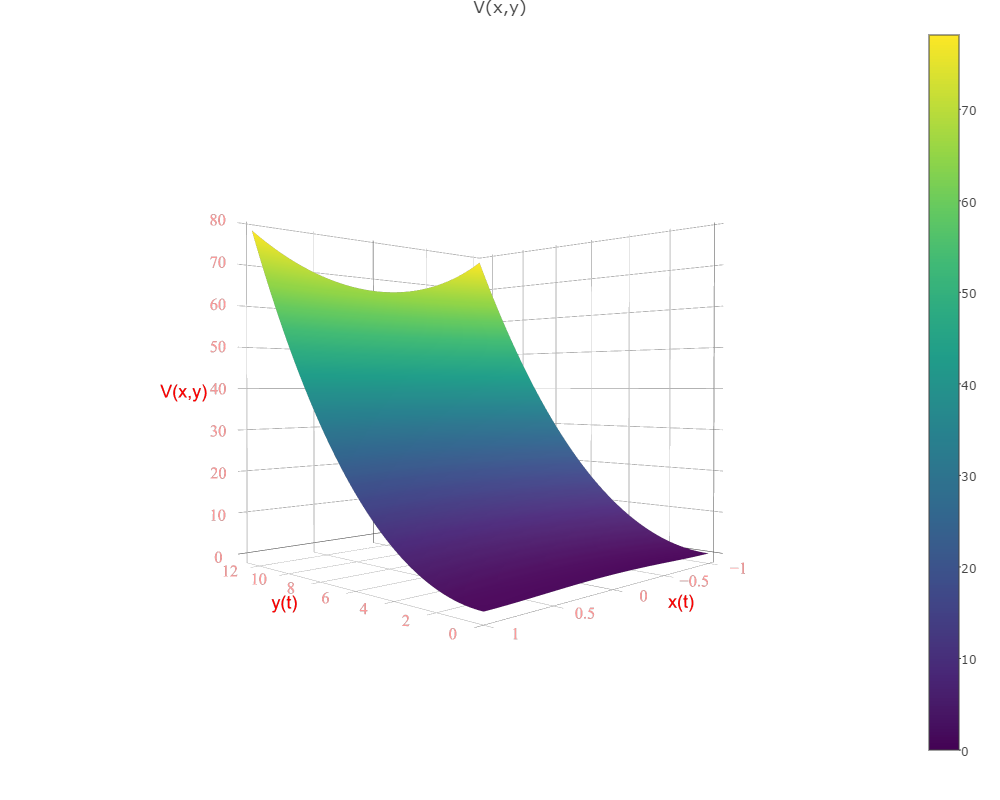
\includegraphics[width=1.0\textwidth]{project_1_g_5_3}
                    }\\%
                    \subfigure[]{%
                    \hspace*{-1.6in}   
                       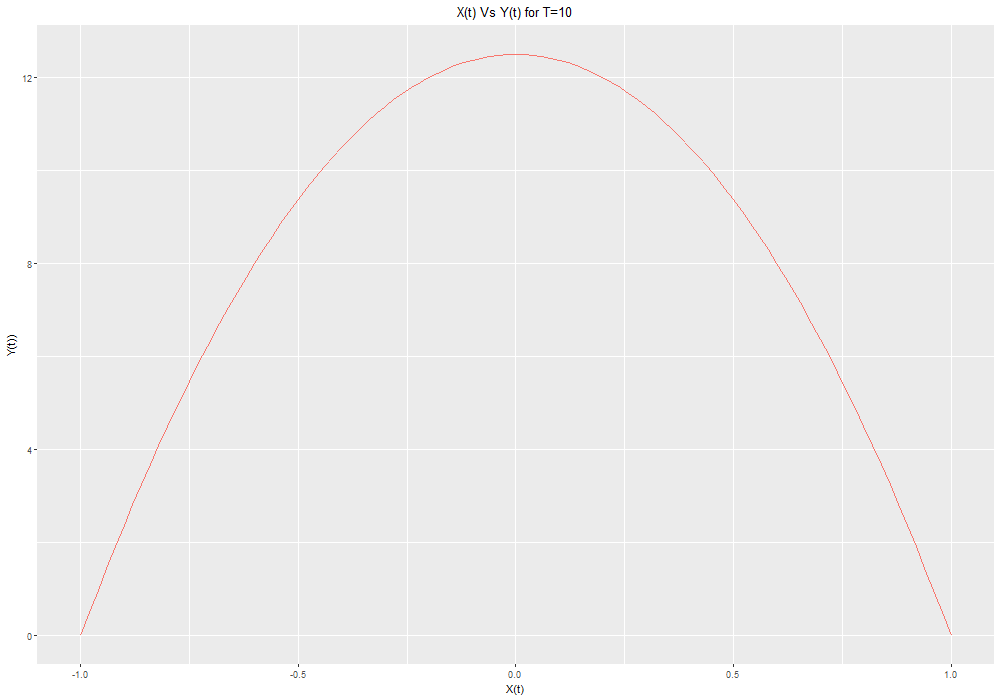
\includegraphics[width=0.75\textwidth]{proj_1_g_xy_t_10}
                    }\\ %  ------- End of the first row ----------------------%
    \end{center}
    \caption{%
     Plot of V(X,Y) Vs X(t)Y(t) and the plot of the solution x(t),y(t) for T=10
     }%
   \label{fig:proj_1_g_t_10}
\end{figure}
}

\FloatBarrier
\subsection{T=20}
{
The iteration for T=20 was performed using a time interval of $h=0.2$. This was done to reduce the matrix size by half in order to speed up execution in MATLAB. The figure $\eqref{fig:proj_1_g_t_20}$ plots the iteration results for $T=20$. Full convergence is not achieved and the process is terminated at 20,000 iterations. While $x$ moves from $(-1 \to 1)$, $y$ takes a still longer path from $0 \to 49.991 \to 0$ for this iteration. The two local minimums at $[-1;0]$ and $[1;0]$ are not very clearly seen in the 3D surface plot of $V(x,y) =  \frac{(1-x^2)^2}{4} + \frac{(y+x^2-1)^2}{2}$ for this range of $x,y$. The $x(t),x(t)$ plot for this iteration shows the longer path taken by this iteration from $[-1;0] \to [1;0]$ It can be seen from the $x(t),y(t)$ plot that in the proximity of $x=0$, y makes a  steep descent towards $[0,1]$ and then a steep ascent back to the trajectory of its earlier path.
\begin{figure}[htbp!]
     \begin{center}
            \hspace*{-1.4in}           
                    \subfigure[]{%
                        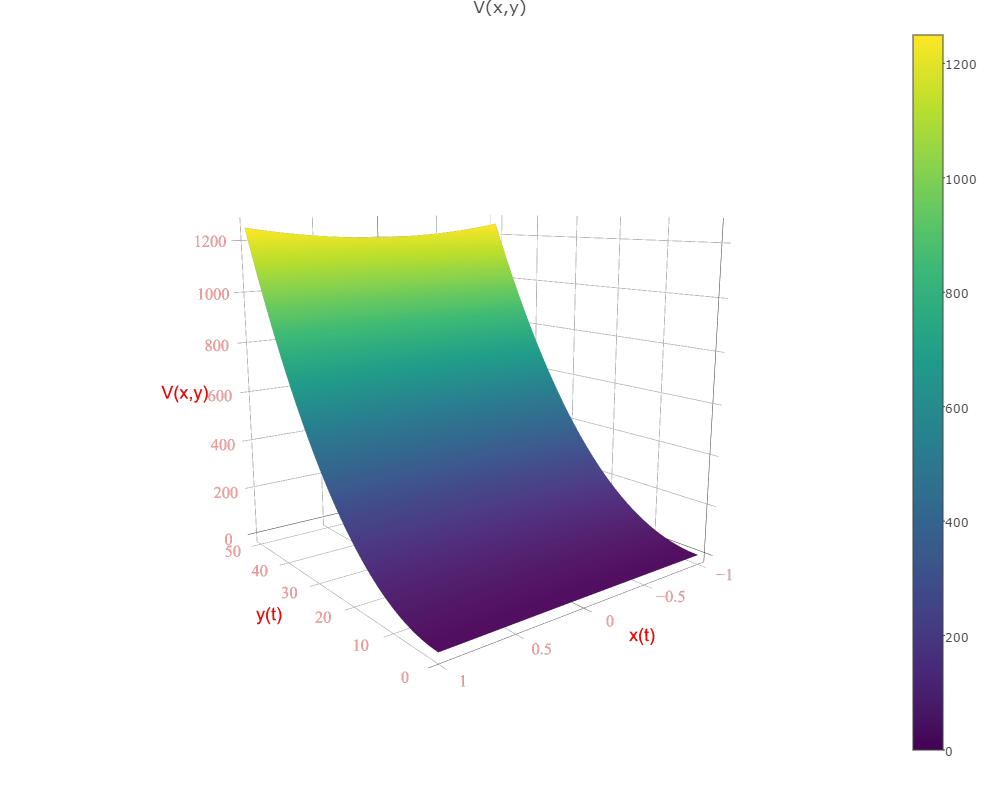
\includegraphics[width=1.0\textwidth]{project_1_g_5_4}
                    }\\%
                    \subfigure[]{%
                    \hspace*{-1.6in}   
                       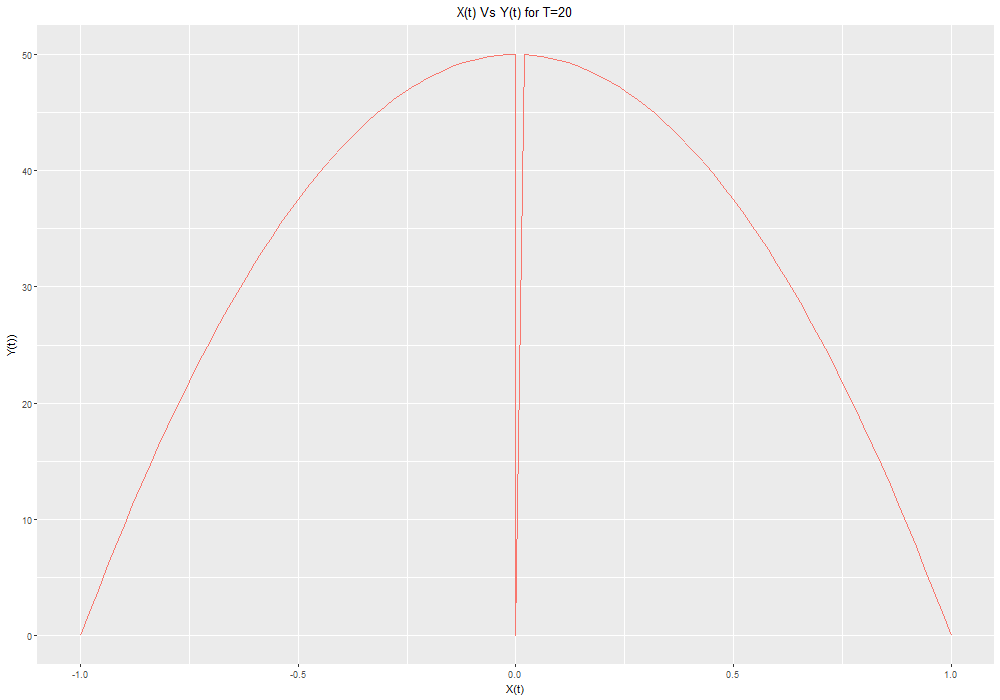
\includegraphics[width=0.75\textwidth]{proj_1_g_xy_t_20}
                    }\\ %  ------- End of the first row ----------------------%
    \end{center}
    \caption{%
     Plot of V(X,Y) Vs X(t)Y(t) and the plot of the solution x(t),y(t) for T=20
     }%
   \label{fig:proj_1_g_t_20}
\end{figure}
}

\FloatBarrier
\subsection{T=100}
{
As with T=20, the iteration for T=100 was performed using a time interval of $h=0.2$. This was done to reduce the matrix size by half in order to speed up execution in MATLAB. The figure $\eqref{fig:proj_1_g_t_100}$ plots the iteration results for $T=100$. Full convergence is not achieved and the process is terminated at 20,000 iterations. While $x$ moves from $(-1 \to 1)$, $y$ takes the longest path of all iterations so far from $0 \to 339.67 \to 0$. The two local minimums at $[-1;0]$ and $[1;0]$ are not very clearly seen in the 3D surface plot of $V(x,y) =  \frac{(1-x^2)^2}{4} + \frac{(y+x^2-1)^2}{2}$ for this range of $x,y$. The $x(t),x(t)$ plot for this iteration shows the longest path taken by this iteration from $[-1;0] \to [1;0]$ As in the T=20 plot, it can also be seen here in the $x(t),y(t)$ plot that in the proximity of $x=0$, y makes a steep descent towards $[0,1]$ and then a steep ascent back to the trajectory of its earlier path.
\begin{figure}[htbp!]
     \begin{center}
            \hspace*{-1.4in}           
                    \subfigure[]{%
                        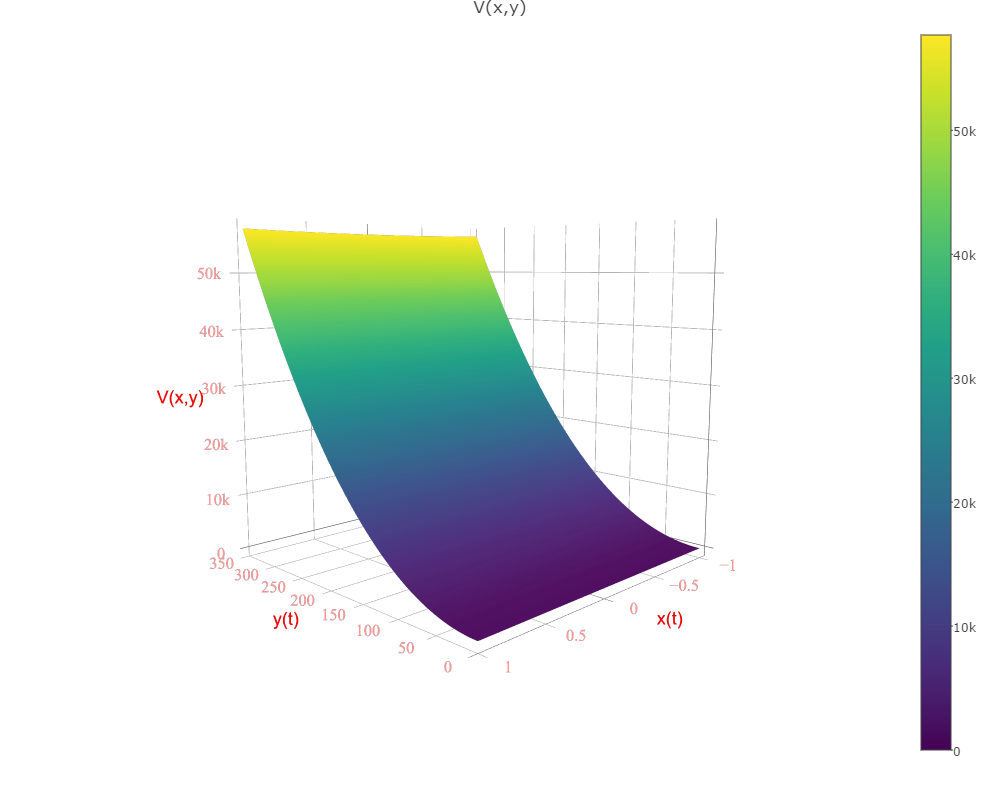
\includegraphics[width=1.0\textwidth]{project_1_g_5_5}
                    }\\%
                    \subfigure[]{%
                    	\hspace*{-1.6in}      
                       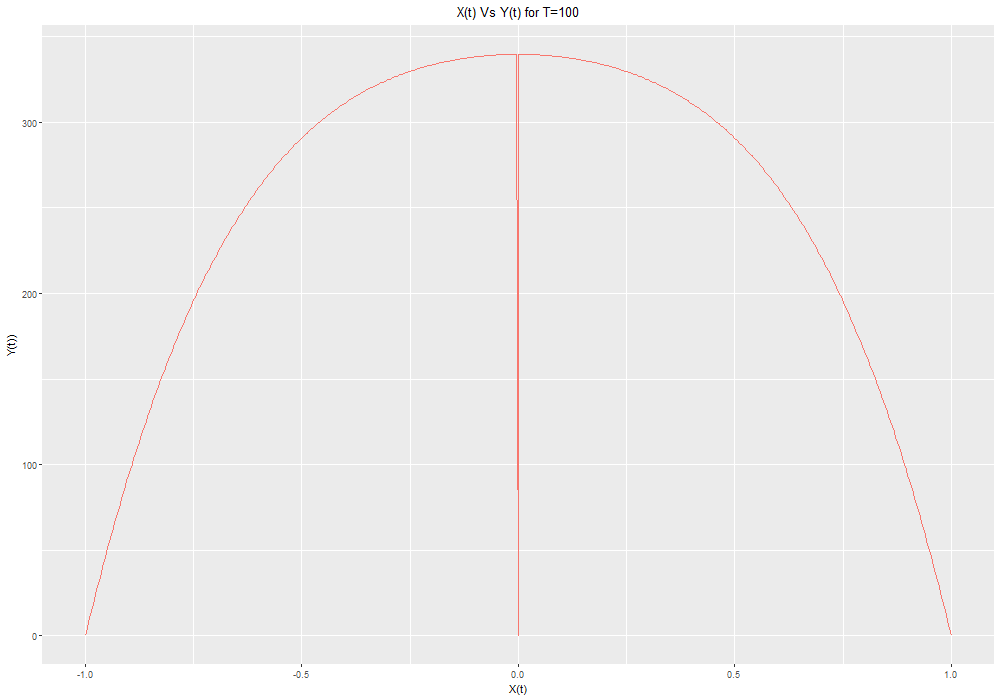
\includegraphics[width=0.75\textwidth]{proj_1_g_xy_t_100}
                    }\\ %  ------- End of the first row ----------------------%
    \end{center}
    \caption{%
     Plot of V(X,Y) Vs X(t)Y(t) and the plot of the solution x(t),y(t) for T=100
     }%
   \label{fig:proj_1_g_t_100}
\end{figure}
}



$\\\\$
\FloatBarrier
\subsection{Comparison of Results for different values of T}
The next three plots compare the performance of the Newtons Iterative Method for the various values of T = $[1,5,10,20,100]$. We first compare the path taken by each iteration using the $x(t)-y(t)$ plots for each of them. Next we compare the different performance metrics for the Newtons Iterative method for these different values of T.
$\\$
\FloatBarrier
\paragraph{x(t)-y(t) Plots}
Figure $\eqref{fig:proj_1_g_xyf}$  plots the $x(t)-y(t)$ path for each value of T on a different facet. Figure $\eqref{fig:proj_1_g_xy}$  plots the $x(t)-y(t)$ path for all the T values on a single plot. From these two plots it can be seen that for larger values of T beyond a certain threshold value, the plot  in the proximity of x=0 tries to take a steep descent to $[0.1]$ and then a steep ascent away from it to continue back to its earlier path. This pattern is seen for T=[100,20] but not seen very conspicuously for T=[1,5,10]. Other than this deviation the paths have a similar pattern for these different values of T. The only difference is that as T gets larger the path gets scaled higher.
{
\begin{figure}[htbp!]
     \begin{center}
            \hspace*{-1.0in}
            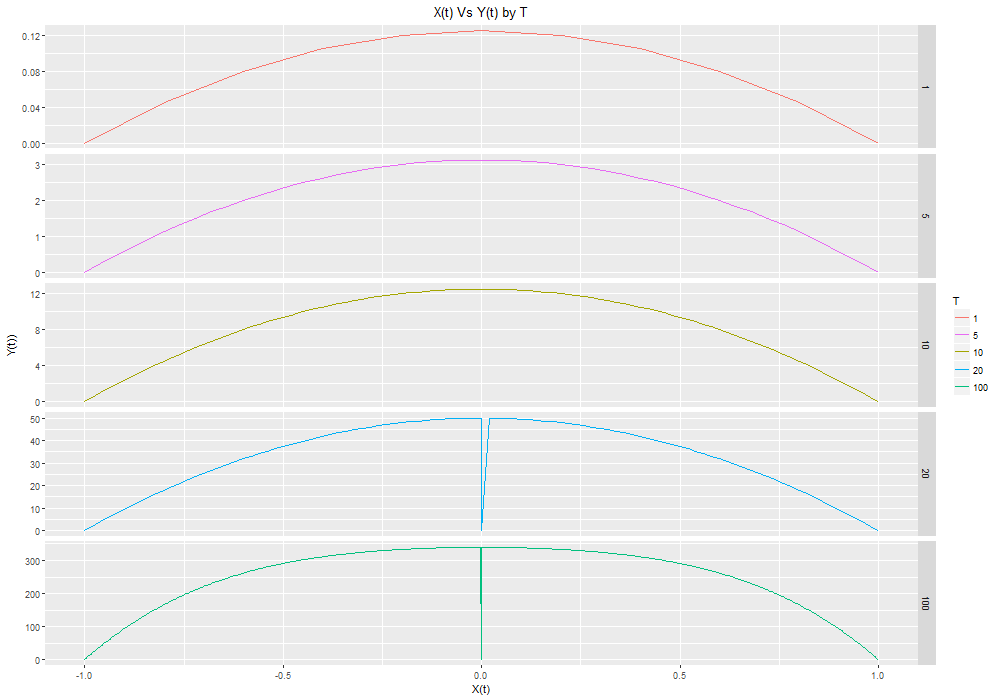
\includegraphics[width=1.35\textwidth]{proj_1_g_xyf}
    \end{center}
    \caption{%
     Solution - Faceted Plot of $x(t)$ Vs $y(t)$ for different values of T
     }%
   \label{fig:proj_1_g_xyf}
\end{figure}
}

\FloatBarrier
{
\begin{figure}[htbp!]
     \begin{center}
            \hspace*{-0.9in}
            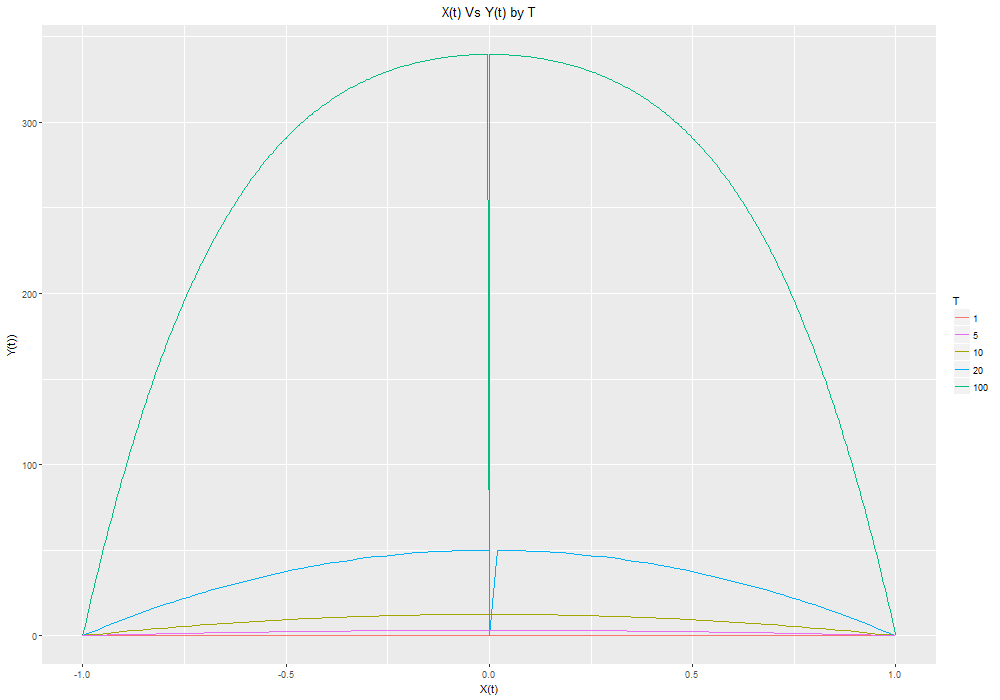
\includegraphics[width=1.2\textwidth]{proj_1_g_xy}
    \end{center}
    \caption{%
     Solution - Single  Plot of $x(t)$ Vs $y(t)$ for different values of T
     }%
   \label{fig:proj_1_g_xy}
\end{figure}
}

$\\$
\FloatBarrier
\paragraph{Performance Metrics}
Figure $\eqref{fig:proj_1_g_perf}$ plots the performance metrics of the Newtons iterative method for each of the cases of T=[1,5,10,20,100]. The following metrics are compared.
\begin{itemize}
\item
Number of iterations
\item
Time taken(Secs)
\item
Residual Norm
\end{itemize}  
As can be seen the performance deteriorates as T is increased. Beyond T=10 the method is slow to converge and has to be ended after 20,000 iterations.  The Time taken increases linearly with T beyond T=20. For values of T less than 20, rapid convergence is achieved within a few seconds. The Residual norm follows a similar pattern to the Time Taken. The Residual norm shows a linear increase as T is increased beyond T=20. For T$<$20, the residual norm is very negligible, which shows good convergence characteristics.

\FloatBarrier
{ 
\begin{figure}[htbp!]
     \begin{center}
            \hspace*{-0.9in}
            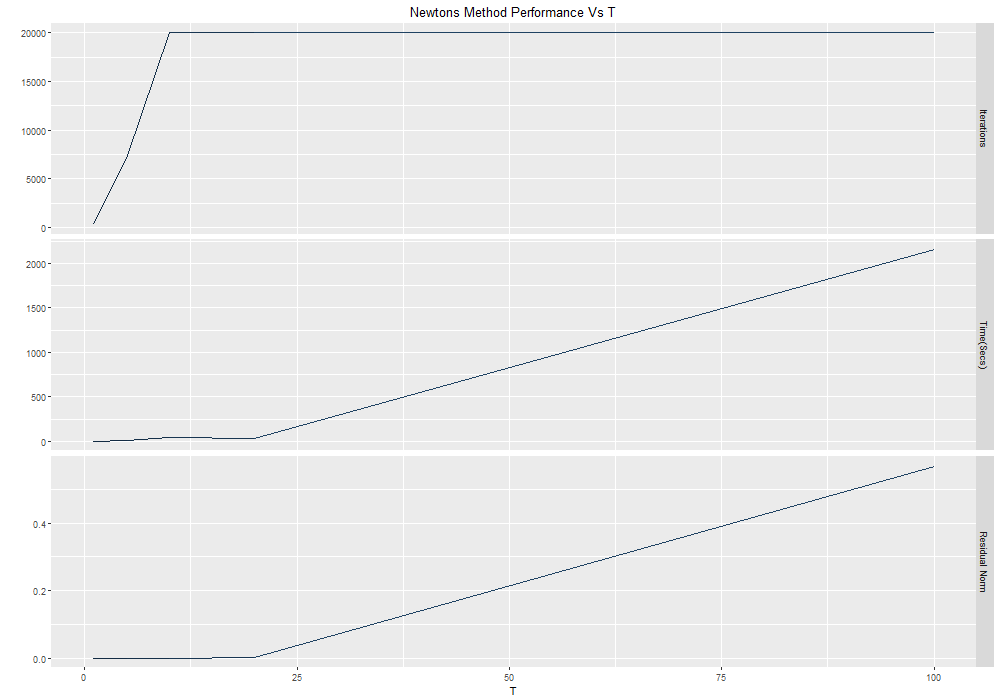
\includegraphics[width=1.2\textwidth]{proj_1_g_perf}
    \end{center}
    \caption{%
     Plots comparing performance of the Newtons method for different values of T
     }%
   \label{fig:proj_1_g_perf}
\end{figure}
}



$\\\\$
\FloatBarrier
\section{Observations}
\label{observations}
\begin{itemize}
\item
A larger value of T results in longer paths and slower convergence. While the performance is good for T=20, the performance deteriorates as T is increased further. The performance of T=100 is far poorer compared with T=20.
\item
For both T=20 and T=100, we see a steep descent and ascent in the proximity of x=0. It appears in this proximity that the (x(t),y(t)) plot tries to get closer to [0,1] and then reverts back to the trajectory of its earlier path. So as T $\rightarrow \infty$ the path will try to intersect with $[0,1]$. For values of T=[1,5,10], no such steep descent in the proximity of x-0 is noticeable. This descent gets pronounced somewhere in the range of $10<T<20$. 
\item
Except for the steep descent seen in the proximity of x=0 for higher values of T, the pattern of the (x(t),y(t)) path is parabolic and similar for the different values of T. The only difference is in the scaling seen in the length of the path as T is increased. The scaling appears to be proportional to the value of T.
\item
The V(X,Y) surface plot shows a slight bulge close to [0.5,0], with local minimum achieved at [-1,0] and [1,0]. As the value of Y increases V(X,Y) keeps increasing rapidly and the bulge is not significant anymore at higher values of y.
\item
Attempting to perform the iterations with a random vector for X which was $\ne  \begin{bmatrix}0\\.\\,\\0\end{bmatrix}$, slowed down the convergence considerably. In some of the cases the residual norm kept increasing showing sings that the process might not converge. With a initial value of $X_{2\times(M-1)} = \begin{bmatrix}0\\.\\,\\0\end{bmatrix}$ the iterative process performed much better tending towards convergence, with convergence rate being inversely related to the value of T.
\end{itemize}


$\\\\$
\FloatBarrier
\section{Scope for Improvement}
\label{improvement}
These iterations where performed with an initial value of $X_{2\times(M-1)} = \begin{bmatrix}0\\.\\,\\0\end{bmatrix}$. However a better initial value than just a zero vector might give better convergence characteristics. One approach would be to use the shooting method to get a initial path starting at the initial boundary value and ending at the final boundary value. The path thus obtained can be used as the initial estimate for X for the Newtons iterative method. This might lead to faster convergence of the Newtons method.

$\\\\$
\FloatBarrier
%\begin{appendices}
\label{appendix}

%\section*{Appendices}
\addcontentsline{toc}{section}{Appendices}
\renewcommand{\thesubsection}{\Alph{subsection}}

\subsection{Source Code - Newtons Method Implementation - MATLAB}
\label{newtons_source}
The MATLAB source code for performing the Newtons Iterative method for solving this system of non linear equations in file $project\_p\_1\_newtons.m$. The source code is also attached below.
\begin{lstlisting}
%
%  ajdsouza31 - DL
%
%  CSE6644 - Project 
% 
% Problem - 1
%
% Implementation of Newtons Method
% For solving a system of Non Linear Equations
% with Boundary Value Condition
%

% clear
clear;

% setting seed for any random number generation
rand('seed', 1234567);
 
% change current folder
cd('C:/wk/odrive/Amazon Cloud Drive/ajays_stuff/georgia_tech_ms/math_cse6644_interative_methods_for_system_of_equations/project');

% tolerance for terminating the iteration
tolerance = 1e-8;

%potential
global V
V=@(x,y) (1-x^2)^2/4+(y+x^2-1)^2/2;

%gradient
global gradV
gradV=@(x,y) [-(1-x^2)*x+2*x*(y+x^2-1);y+x^2-1];

%Hessian
global HessV
HessV=@(x,y) [-1+3*x^2+2*(y+x^2-1)+4*x^2 2*x;2*x 1];

%F_x
global F_x
F_x=@(x,y) (27*x^5 - 34*x^3 + 7*x  + ...
    24*x^3*y + 4*x*y^2 - 10*x*y);

%F_y
global F_y
F_y=@(x,y) ( 6*x^4 - 5*x^2 + ...
    4*x^2*y + y - 1);

%dF_1_dx
global dF_1_dx
dF_1_dx=@(x,y) (135*x^4 - 102*x^2 + 7 + 72*x^2*y + 4*y^2-10*y);

%dF_2_dx
global dF_2_dx
dF_2_dx=@(x,y) (24*x^3 - 10*x + 8*x*y);

%dF_1_dy
global dF_1_dy
dF_1_dy=@(x,y) (24*x^3 + 8*x*y - 10*x);

%dF_2_dy
global dF_2_dy
dF_2_dy=@(x,y) (4*x^2 + 1);

%initial value
global X0
X0=[-1;0];

%endvalue
global XT
XT=[1;0];

% The list of T to be used
% T= M*dh => T= n*dh
Tl = [1,5,10,20,100];


% time interval size for each T
% T = M*dh => T= n*dh
dhL = [0.1,0.1,0.1,0.2,0.2];

% color for plotting for each T
colr = ['r','g','b','k','m'];

% save x and y for plotting
Xsave = zeros((max(Tl)/min(dhL))+1,length(Tl));
Ysave = zeros((max(Tl)/min(dhL))+1,length(Tl));

% save performance statistics
perfMetrics = zeros(length(Tl),5);

% run newtons method for each T
for Ti = 1:length(Tl)
    
    % get the T
    T = Tl(Ti);
    
    % get the timestamp for this T
    dh = dhL(Ti);
    
    % no of intervals M, so points is M+1
    % T = M*dh => T= n*dh
    % No o points is M+1 from 0..M or in matlab 1...M+1
    M = T/dh;
  
    
    % Set up for newtons method for each T        
    %Ybar
    Ybar = zeros(2*(M-1),1);
    Ybar(1,1) = -1;
    Ybar(2*(M-2)+1,1) = 1;
    
    % A
    A = zeros(2*(M-1));
    % check if matrix is positive definite - P is 0
    [~,p] = chol(A);
    
    for i=1:(M-1)
        
        idx = (i-1)*2;
        
        A(idx+1,idx+1) = 2;
        A(idx+2,idx+2) = 2;
        
        if ( i > 1 )
            A(idx+1,idx-1) = -1;
            A(idx+2,idx) = -1;
        end
        
        if ( i < (M-1) )
            A(idx+1,idx+3) = -1;
            A(idx+2,idx+4) = -1;
        end
        
    end
    
    
    % X
    % initilized to 0 
    X =  zeros(2*(M+1),1);
    X(1,1) = -1;
    X((2*M)+1,1) = 1;
    %X(3:2*M,1) = rand(2*(M-1),1)-(1/2);
    
    
    %RHS F(X_i)
    F = zeros(2*(M-1),1);
    
    for i=1:(M-1)
        idx = (i-1)*2;
        F(idx+1:idx+2,1) = ...
            HessV(X(idx+2),X(idx+3))*gradV(X(idx+2),X(idx+3));
    end
    
    
    %Jacobian
    % J = A+h^2J(F(X))
    J = zeros(2*(M-1));
    
    for i=1:(M-1)
        
        idx = (i-1)*2;
        
        J(idx+1:idx+2,idx+1:idx+2) = ...
            dh^2*([dF_1_dx(X(idx+2),X(idx+3)),dF_1_dy(X(idx+2),X(idx+3));
            dF_2_dx(X(idx+2),X(idx+3)),dF_2_dy(X(idx+2),X(idx+3))]);
        
        
        J(idx+1,idx+1) = 2 + J(idx+1,idx+1);
        J(idx+2,idx+2) = 2 + J(idx+1,idx+1);
        
        if ( i > 1 )
            J(idx+1,idx-1) = J(idx+1,idx-1)-1;
            J(idx+2,idx) = J(idx+2,idx)-1;
        end
        
        if ( i < (M-1) )
            J(idx+1,idx+3) = J(idx+1,idx+3)-1;
            J(idx+2,idx+4) = J(idx+2,idx+4)-1;
        end
    end
        
    %start time in secs
    startTime = datevec(now);
    
    % Newton Method - Begin Iterations
    
    % get the initial residue to start the loop
    b = A*X(3:2*M) + dh^2*F - Ybar;
    
    iterations = 0;
    while(max(abs(b))>tolerance)
        
        % compute the new x from old x
        % as x(t+1) = x(t) - inv(Jacobian)*b
        X(3:2*M) = X(3:2*M) - inv(J)*b;

        % get the reside b with the new x
        b = A*X(3:2*M) + dh^2*F - Ybar;
        
        iterations = iterations + 1;
        
        % limit on iterations 
        if iterations > 20000
            fprintf('Reached Limit Breaking \n T=%d , Iteration:%d  - norm:%f\n',...
                 T,iterations,norm(b));
            break;
        end
        
        % print progress of the iterations
        if rem(iterations,50) == 0
             fprintf('T=%d , Iteration:%d  - norm:%f\n',...
                 T,iterations,norm(b));
        end
    end
    
    % clear what we do not bneed ad newtons method has exited
    % for this T
    clear J;
    clear A;
    clear F;
    clear Ybar;
    
    %time taken in secs
    endTime = datevec(now);
    
    fprintf('T= %d\n',T);
    fprintf('Time Taken(s) %f\n',etime(endTime,startTime));
    fprintf('Converging Norm %f\n\n\n',norm(b));
    
    % get the X and Y values into two different arrays
    Y=X(2:2:end);
    X(2:2:end)=[];
    
    % save them to a struct whcih keeps teach of X,Y values for
    % all T , will save them to file later for plotting
    Xsave(1:length(X),Ti) = X;
    Ysave(1:length(Y),Ti) = Y;
    
    % save the performance metric fro this T
    % will be saved to file for plotting
    perfMetrics(Ti,:) = [T,iterations,...
       etime(endTime,startTime),norm(b),dh];

    % A trivial plot for checking
    plot(X,Y,'color',colr(Ti));
    hold on;

    % clear the X,Y from newtons as this has been saved and iteration
    % is complete
    clear X;
    clear Y;
    
    %[X,Y] = meshgrid(-1:.1:1);
    %mesh(X,Y,V(X,Y))
      
end


% save the results to a csv file, can be read by R to plot in by ggplot
fname = sprintf('project_1_x.csv');
csvwrite(fname,Xsave);


% save the results to a csv file, can be read by R to plot in by ggplot
fname = sprintf('project_1_y.csv');
csvwrite(fname,Ysave);


% save the results to a csv file, can be read by R to plot in by ggplot
fname = sprintf('project_1_perf.csv');
csvwrite(fname,perfMetrics);


%--------------------------END ------------------------------------

\end{lstlisting}

$\\\\$
\subsection{Source Code for Plotting Results = R}
\label{plotting_source}
The R source code for plotting the results and solution from the Newtons Iterative method is implemented in file $project\_p\_1\_plot\_csv\_results.R$. The source code is also attached below.
\begin{lstlisting}
require(ggplot2)
require(reshape)
require(gridExtra)
library(reshape2)
library(plotly)
require(webshot)
library(htmlwidgets)


# clear everything
rm(list = ls())

set.seed(100)

setwd(
  "C:/wk/odrive/Amazon Cloud Drive/ajays_stuff/georgia_tech_ms/math_cse6644_interative_methods_for_system_of_equations/project"
)

sink("project_1_script_output.txt",
     append = FALSE,
     split = TRUE)
sink()


# read the matlab results into R dataframe
xDf <-
  read.csv(paste("project_1_x", ".csv", sep = ""),
           header = FALSE)

# read the matlab results into R dataframe
yDf <-
  read.csv(paste("project_1_y", ".csv", sep = ""),
           header = FALSE)


# read the matlab results into R dataframe
pDf <-
  read.csv(paste("project_1_perf", ".csv", sep = ""),
           header = FALSE)


colnames(pDf) <- c('T','Iterations','Time(Secs)','Residual Norm','h')

rownames(xDf) <- 1:length(xDf[['V1']])
rownames(yDf) <- 1:length(xDf[['V1']])  

xM <- data.matrix(xDf)
yM <- data.matrix(yDf)


# rows in each x,y
M <- as.vector((pDf$T/.1)+1)

# melt the performance data for gg plot of the data frame with pivot as id
xDf$id <- 1:length(xDf[['V1']])
yDf$id <- 1:length(xDf[['V1']])

# calculate V


# GG Plot of X,Y for each T
dat <- setNames(lapply(1:length(M), function(x) cbind(x=xDf[1:M[x],x], y=yDf[1:M[x],x])), as.vector(pDf$T))

list.names <- names(dat)
lns <- sapply(dat, nrow)
dat <- as.data.frame(do.call("rbind", dat))
dat$group <- rep(list.names, lns)

# Plot x(t), y(t)

gg_color_hue <- function(n) {
  hues = seq(15, 375, length = n + 1)
  hcl(h = hues, l = 65, c = 100)[1:n]
}

par(
  mfrow = c(1, 1),
  oma = c(0, 0, 2, 0),
  lab = c(2, 5, 3),
  lwd = 1,
  pch = 19
)

g1 <- ggplot(dat, aes(x = x, y = y)) +
  labs(x = "X(t)",
       y = "Y(t))",
       colour = "")  +
  geom_line(linetype="solid",aes(colour = group)) + 
  ggtitle(paste("X(t) Vs Y(t) by T",sep="")) +
  theme(plot.title = element_text(hjust = 0.5)) +
  scale_color_manual(name="T",breaks=pDf$T,values=gg_color_hue(length(M)))

grid.arrange(g1)

dev.copy(filename = paste("proj_1_g_xy", ".png", sep = ""),
         device=png, width=1000,height=700)

dev.off()


# Plot individual plots for each T
for( i in 1:length(pDf$T)) {
  
  par(
    mfrow = c(1, 1),
    oma = c(0, 0, 2, 0),
    lab = c(2, 5, 3),
    lwd = 1,
    pch = 19
  )
  
  gi <- ggplot(dat[which(dat$group == pDf$T[i] ),], 
               aes(x = x, y = y),group=pDf$T[i]) +
    labs(x = "X(t)",
         y = "Y(t))",
         colour = "")  +
    geom_line(linetype="solid",aes(colour = group)) + 
    ggtitle(paste("X(t) Vs Y(t) for T=",pDf$T[i],sep="")) +
    theme(plot.title = element_text(hjust = 0.5),legend.position="none")
  
  grid.arrange(gi)
  
  dev.copy(filename = paste("proj_1_g_xy_t_",pDf$T[i], ".png", sep = ""),
           device=png, width=1000,height=700)
  
  dev.off()
  
}

# Plot x(t), y(t) as facet

par(
  mfrow = c(1, 1),
  oma = c(0, 0, 2, 0),
  lab = c(2, 5, 3),
  lwd = 1,
  pch = 19
)

# arrange facets in order
dat$group_f <- factor(dat$group,levels=pDf$T)

g2 <- ggplot(dat, aes(x=x, y=y, group = 1)) +
  geom_line(aes(colour = group)) +
  facet_grid(group_f~., scales = "free_y") +
  labs(x = "X(t)",
       y = "Y(t))",
       colour = "") +
  ggtitle(paste("X(t) Vs Y(t) by T",sep="")) +
  theme(plot.title = element_text(hjust = 0.5)) +
  scale_color_manual(name="T",breaks=pDf$T,values=gg_color_hue(length(M)))


grid.arrange(g2)

dev.copy(filename = paste("proj_1_g_xyf", ".png", sep = ""),
         device=png, width=1000,height=700)

dev.off()




# Plot of the performance for the different T's

#melt with method name as pivot
molten <-
  melt(
    pDf[, c('T', 'Iterations', 'Time(Secs)', 'Residual Norm')],
    id.vars = c('T'),
    measure.vars = c('Iterations', 'Time(Secs)', 'Residual Norm'),
    variable_name = 'series'
  )

par(
  mfrow = c(1, 1),
  oma = c(0, 0, 2, 0),
  lab = c(2, 5, 3),
  lwd = 1,
  pch = 19
)

klabs <- c(pDf$T)


g3 <- ggplot(molten, aes(x=T, y=value, group = 1)) +
  geom_line(aes(colour = T)) +
  facet_grid(series~., scales = "free_y") +
  labs(x = "T",
       y = "",
       colour = "") +
  ggtitle(paste("Newtons Method Performance Vs T",sep="")) +
  theme(plot.title = element_text(hjust = 0.5),legend.position="none") 


grid.arrange(g3)

dev.copy(png,
         filename = "proj_1_g_perf.png",
         width = 1000,
         height = 700)

dev.off()



# 3D Plot of V(x,y)

# Use the one with the max x,y
#vI <- which(M==max(M))

# v(x,y) function
V_x_y <- function(x,y) {
  ((1 - x^2)^2)/4 + ((y + x^2 - 1)^2)/2 
}


for (vI in 1:length(M)) {
  
  
  mX <- min(xDf[vI])
  iX <- max(xDf[vI])
  
  mX <- -1
  iX <- 1
  
  mY <- min(yDf[vI])
  iY <- max(yDf[vI])
  
  xx <- seq(mX, iX, length.out = 100)  
  yy <- seq(mY, iY, length.out = 100)   
  
  
  zz <- data.frame(outer(xx, yy, V_x_y))  
  
  colnames(zz) <- yy
  rownames(zz) <- xx
  
  zz <- as.matrix(zz)
  # Create lists for axis properties
  f1 <- list(
    family = "Arial, sans-serif",
    size = 18,
    color = "red")
  
  f2 <- list(
    family = "Old Standard TT, serif",
    size = 14,
    color = "#ff9999")
  
  axis <- list(
    titlefont = f1,
    tickfont = f2,
    showgrid = T
  )
  
  xaxis <- c(list(title='x(t)'),axis)
  yaxis <- c(list(title='y(t)'),axis)
  zaxis <- c(list(title='V(x,y)'),axis)
  
  scene = list(
    xaxis = yaxis,
    yaxis = xaxis,
    zaxis = zaxis,
    camera = list(eye = list(x = -1.65, y = 1.25, z = 1.55)))
  
  
  
  ply <- plot_ly(y=xx,x=yy,z=zz, type = "surface", size = I(3),
                 width=1000,
                 height=800) %>% 
    layout(title = paste("V(x,y)"), scene = scene)  
  
  
  saveWidget(as.widget(ply), paste("project_1_g_5_",vI ,".html", sep = ""))
  
  #rm(ply)
}


\end{lstlisting}


%\end{appendices}



$\\\\$
%\addcontentsline{toc}{section}{References}
\bibliographystyle{unsrt}
\bibliography{sample}
%\bibliographystyle{plain}
% Generate the bibliography.
\begin{thebibliography}{9}

\bibitem{kelly_1995}
  Kelly C.T.,
  \emph{Iterative Methods for Linear and Nonlinear Equations},
  Society for Industrial and Applied Mathematics, Philadelphia,
  1995.

\end{thebibliography}

\end{document}